\documentclass[aspectratio=169]{beamer}
\usepackage[utf8]{inputenc}
\usepackage{booktabs}
\usepackage{adjustbox}
\usepackage{amsmath,amssymb,amsthm}
\usepackage{mathtools}
\usepackage{subcaption}
\usepackage{tikz}
\usepackage{tikz-cd}
\usepackage{float}
\mathtoolsset{showonlyrefs}

\newcommand{\authorname}{Gonzalo Ortega Carpintero}
\newcommand{\tutorname}{Manuel Mellado Cuerno}
\newcommand{\institution}{Universidad Autónoma de Madrid}
\newcommand{\projecttitle}{Structure and Stability Theorems in Topological Data Analysis

Draft}

\newcommand{\dgmp}{\operatorname{Dgm}_p}
\newcommand{\dgmi}{\operatorname{Dgm}_\infty}
\newcommand{\costp}{\operatorname{cost}_p}
\newcommand{\costi}{\operatorname{cost}_\infty}
\newcommand{\wdp}{\omega_p}
\newcommand{\wdi}{\omega_\infty}
\newcommand{\twdp}{\tilde \omega_p}
\newcommand{\twdi}{\tilde \omega_\infty}
\newcommand{\p}{\mathcal P}
\newcommand{\B}{\mathcal B}
\newcommand{\T}{T_\#}
\newcommand{\N}{\mathbb N}
\newcommand{\Z}{\mathbb Z}
\newcommand{\R}{\mathbb R}
\newcommand{\e}{\varepsilon}
\newcommand{\upr}{\mathbb{R}_<^2}

\newcommand{\barc}{\operatorname{Bar}}
\newcommand{\im}{\operatorname{im}}

\newcommand{\db}{d_{\operatorname{bot}}}

\usetheme{Madrid}

\definecolor{mycolor}{rgb}{0.5, 0.5, 0.75}
\definecolor{green}{rgb}{0.3, 0.7, 0.3}
\definecolor{grey}{rgb}{0.4, 0.4, 0.4}
\usecolortheme[named=mycolor]{structure}

\useoutertheme{infolines} % Alternatively: miniframes, infolines, split

\setbeamercolor{palette primary}{bg=green,fg=white} % Titulo, derecha
\setbeamercolor{palette secondary}{bg=green,fg=white} % Medio
\setbeamercolor{palette tertiary}{bg=green,fg=white} % Izquierda
\setbeamercolor{structure}{fg=grey} % Fondos y secciones


\title{Structure and Stability Theorems}
\subtitle{in Topological Data Analysis}
\author{Master's Final Thesis}
\institute{Author: \authorname \and Advisor (UPM): Jaime Santos Rodríguez \and Advisor (UAM): Luis Guijarro Santamaría}
\titlegraphic{
\includegraphics[height=1cm]{../figures/marcaUAM_AhorizontalColor_imp.pdf}}
\date{Thursday, July 3, 2025}

\setbeamertemplate{footline}{
  \leavevmode%
  \hbox{%
    \begin{beamercolorbox}[wd=0.33\paperwidth,ht=2.5ex,dp=1ex,center]{author in head/foot}%
      \usebeamerfont{author in head/foot}\authorname
    \end{beamercolorbox}%
    \begin{beamercolorbox}[wd=0.33\paperwidth,ht=2.5ex,dp=1ex,center]{title in head/foot}%
      \usebeamerfont{title in head/foot}Structure and Stability Theorems in TDA
    \end{beamercolorbox}%
    \begin{beamercolorbox}[wd=0.24\paperwidth,ht=2.5ex,dp=1ex,center]{title in head/foot}%
      \usebeamerfont{title in head/foot}Thursday, July 3, 2025
    \end{beamercolorbox}%
    \begin{beamercolorbox}[wd=0.1\paperwidth,ht=2.5ex,dp=1ex,right]{date in head/foot}%
      \usebeamerfont{date in head/foot}\insertframenumber{} / \inserttotalframenumber \hspace{1em}
    \end{beamercolorbox}%
  }%
}

\begin{document}

\frame[plain]{\titlepage}

\AtBeginSection[]
{
  \begin{frame}{Contents}
    \tableofcontents[currentsection]
  \end{frame}
}

\section{Preliminaries}

\subsection{Persistent homology}

\begin{frame}
  \begin{figure}
        \centering
        \begin{subfigure}[b]{0.45\linewidth}
            \centering
            \begin{tikzpicture}[line cap=round, line join=round, x=1cm, y=1cm, scale=0.8]
                \clip (-0.5, 0) rectangle (5, 3.5);
                \coordinate (a) at (0.21, 0.14);
                \coordinate (b) at (0.62, 2.82);
                \coordinate (c) at (2.01, 1.32);
                \coordinate (d) at (4.23, 2.23);
                \draw (c) -- (d);
                \foreach \point/\pos in {a/above left, b/above left, c/below right, d/above right}
                    \draw[fill=black] (\point) circle (1pt) node[\pos] {$\point$};
            \end{tikzpicture}
            \caption*{$F_0 K$}
        \end{subfigure}
        \begin{subfigure}[b]{0.45\linewidth}
            \centering
            \begin{tikzpicture}[line cap=round, line join=round, x=1cm, y=1cm, scale=0.8]
                \clip (-0.5, 0) rectangle (5, 3.5);
                \coordinate (a) at (0.21, 0.14);
                \coordinate (b) at (0.62, 2.82);
                \coordinate (c) at (2.01, 1.32);
                \coordinate (d) at (4.23, 2.23);
                \draw (c) -- (d) -- (b) -- cycle;
                \foreach \point/\pos in {a/above left, b/above left, c/below right, d/above right}
                    \draw[fill=black] (\point) circle (1pt) node[\pos] {$\point$};
            \end{tikzpicture}
            \caption*{$F_1 K$}
        \end{subfigure}
        \begin{subfigure}[b]{0.45\linewidth}
            \centering
            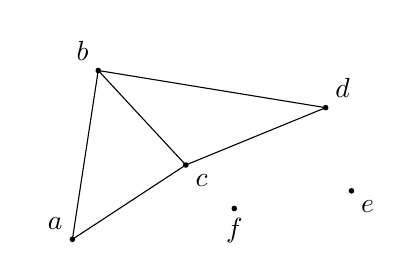
\begin{tikzpicture}[line cap=round, line join=round, x=1cm, y=1cm, scale=0.8]
                \clip (-0.5, 0) rectangle (5, 3.5);
                \coordinate (a) at (0.21, 0.14);
                \coordinate (b) at (0.62, 2.82);
                \coordinate (c) at (2.01, 1.32);
                \coordinate (d) at (4.23, 2.23);
                \coordinate (e) at (4.64, 0.91);
                \coordinate (f) at (2.78, 0.63);
                \draw (a) -- (b) -- (c) -- cycle;
                \draw (c) -- (d) -- (b);
                \foreach \point/\pos in {a/above left, b/above left, c/below right, d/above right, e/below right, f/below}
                    \draw[fill=black] (\point) circle (1pt) node[\pos] {$\point$};
            \end{tikzpicture}
            \caption*{$F_2 K$}
        \end{subfigure}
        \begin{subfigure}[b]{0.45\linewidth}
            \centering
            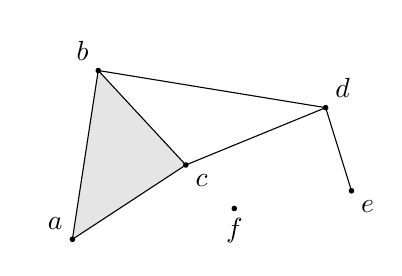
\begin{tikzpicture}[line cap=round, line join=round, x=1cm, y=1cm, scale=0.8]
                \clip (-0.5, 0) rectangle (5, 3.5);
                \coordinate (a) at (0.21, 0.14);
                \coordinate (b) at (0.62, 2.82);
                \coordinate (c) at (2.01, 1.32);
                \coordinate (d) at (4.23, 2.23);
                \coordinate (e) at (4.64, 0.91);
                \coordinate (f) at (2.78, 0.63);
                \fill[fill=black, fill opacity=0.1] (a) -- (b) -- (c) -- cycle;
                \draw (a) -- (b) -- (c) -- cycle;
                \draw (c) -- (d) -- (b);
                \draw (d) -- (e);
                \foreach \point/\pos in {a/above left, b/above left, c/below right, d/above right, e/below right, f/below}
                    \draw[fill=black] (\point) circle (1pt) node[\pos] {$\point$};
            \end{tikzpicture}
            \caption*{$F_3 K$}
        \end{subfigure}
        \caption{Four step filtration of a simplicial complex $K$.}
    \end{figure}
\end{frame}

\begin{frame}
  \frametitle{Preliminaries}
  \framesubtitle{Persistent homology}

  \begin{block}{Definition (Persistence module)}
    Let $\F$ be a field and let $T$ be a totally ordered set. Let $ V = \{V_t\}_{t \in T} $ be a collection of $F$-vector spaces. A $T$-indexed {\bf persistence module} is a pair $ (V, \pi) $ such that $ \pi = \{ \pi_{s \leq t} \} $ is a collection of linear maps $ \pi_{s \leq t}\colon V_s \rightarrow V_t $ that verifies that for all $ r, s, t \in T $,
    \begin{equation}
        \pi_{r \leq s} \circ \pi_{s \leq t} = \pi_{r \leq t}.
    \end{equation}
  \end{block}
\end{frame}

\begin{frame}
  \frametitle{Preliminaries}
  \framesubtitle{Persistent homology}

  \begin{block}{Definition $\delta$-interleaved modules}
    Let $ (V, \pi), (W, \theta) $ be two persistence modules and let $ \delta > 0 $. $ V $ and $ W $ are {\bf $\delta$-interleaved } if there exists two persistence module morphisms $ \phi \colon V \to W_\delta $ and $ \psi \colon W \to V_\delta $ such that the following diagrams commute:
  \end{block}


  \centering
  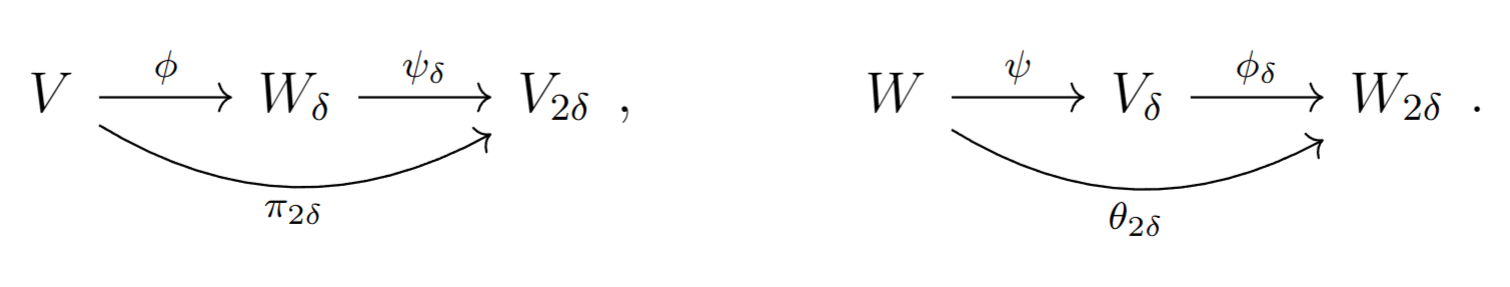
\includegraphics[width=0.8\linewidth]{../figures/diagrams.png}

\end{frame}

\begin{frame}
  \frametitle{Preliminaries}
  \framesubtitle{Persistent homology}
  \begin{block}{Definition (Interleaving distance)}
    Let $ (V, \pi) $ and $ (W, \theta) $ be two tame persistence modules. The {\bf interleaving distance} between them is defined as
    \begin{equation}
        \di(V, W) \coloneq \inf \{ \delta > 0 \mid V \text{ and } W \text{ are } \delta\text{-interleaved}\}.
    \end{equation}
  \end{block}
\end{frame}

\begin{frame}
  \frametitle{Preliminaries}
  \framesubtitle{Persistent homology}
  \begin{block}{Definition (Barcode)}
        A {\bf barcode} $B$ is a finite multiset of intervals. That is, a collection $\{(I_i, m_i)\}$ of intervals $I_i$ with multiplicities $m_i \in N$, where each interval $ I_i $ is either finite of the form $(a, b]$ or infinite of the form $(a, \infty)$. Each interval $I_i$ is named to be a {\bf bar} of $B$. The first number, $ a $ is named the {\bf birth} of the barcode and is second number is its {\bf death}.
  \end{block}
\end{frame}

\begin{frame}
  \begin{figure}
  \centering
        \begin{subfigure}[b]{0.2\linewidth}
            \centering
            \begin{tikzpicture}[line cap=round, line join=round, x=1cm, y=1cm, scale=0.4]
                \clip (-0.5, 0) rectangle (5, 3.5);
                \coordinate (a) at (0.21, 0.14);
                \coordinate (b) at (0.62, 2.82);
                \coordinate (c) at (2.01, 1.32);
                \coordinate (d) at (4.23, 2.23);
                \draw (c) -- (d);
                \foreach \point/\pos in {a/above left, b/above left, c/below right, d/above right}
                    \draw[fill=black] (\point) circle (1pt);
            \end{tikzpicture}
            \caption*{$F_0 K$}
        \end{subfigure}
        \begin{subfigure}[b]{0.2\linewidth}
            \centering
            \begin{tikzpicture}[line cap=round, line join=round, x=1cm, y=1cm, scale=0.4]
                \clip (-0.5, 0) rectangle (5, 3.5);
                \coordinate (a) at (0.21, 0.14);
                \coordinate (b) at (0.62, 2.82);
                \coordinate (c) at (2.01, 1.32);
                \coordinate (d) at (4.23, 2.23);
                \draw (c) -- (d) -- (b) -- cycle;
                \foreach \point/\pos in {a/above left, b/above left, c/below right, d/above right}
                    \draw[fill=black] (\point) circle (1pt);
            \end{tikzpicture}
            \caption*{$F_1 K$}
        \end{subfigure}
        \begin{subfigure}[b]{0.2\linewidth}
            \centering
            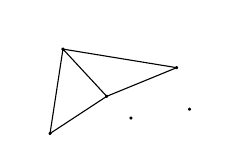
\begin{tikzpicture}[line cap=round, line join=round, x=1cm, y=1cm, scale=0.4]
                \clip (-0.5, 0) rectangle (5, 3.5);
                \coordinate (a) at (0.21, 0.14);
                \coordinate (b) at (0.62, 2.82);
                \coordinate (c) at (2.01, 1.32);
                \coordinate (d) at (4.23, 2.23);
                \coordinate (e) at (4.64, 0.91);
                \coordinate (f) at (2.78, 0.63);
                \draw (a) -- (b) -- (c) -- cycle;
                \draw (c) -- (d) -- (b);
                \foreach \point/\pos in {a/above left, b/above left, c/below right, d/above right, e/below right, f/below}
                    \draw[fill=black] (\point) circle (1pt);
            \end{tikzpicture}
            \caption*{$F_2 K$}
        \end{subfigure}
        \begin{subfigure}[b]{0.2\linewidth}
            \centering
            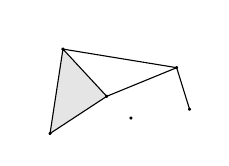
\begin{tikzpicture}[line cap=round, line join=round, x=1cm, y=1cm, scale=0.4]
                \clip (-0.5, 0) rectangle (5, 3.5);
                \coordinate (a) at (0.21, 0.14);
                \coordinate (b) at (0.62, 2.82);
                \coordinate (c) at (2.01, 1.32);
                \coordinate (d) at (4.23, 2.23);
                \coordinate (e) at (4.64, 0.91);
                \coordinate (f) at (2.78, 0.63);
                \fill[fill=black, fill opacity=0.1] (a) -- (b) -- (c) -- cycle;
                \draw (a) -- (b) -- (c) -- cycle;
                \draw (c) -- (d) -- (b);
                \draw (d) -- (e);
                \foreach \point/\pos in {a/above left, b/above left, c/below right, d/above right, e/below right, f/below}
                    \draw[fill=black] (\point) circle (1pt);
            \end{tikzpicture}
            \caption*{$F_3 K$}
        \end{subfigure}
      \end{figure}
  \vspace{-1cm}
  \begin{figure}
        \centering
        \begin{subfigure}[b]{0.4\linewidth}
            \centering
            \begin{tikzpicture}[line cap=round, line join=round, x=1cm, y=1cm, scale=0.8]
                \clip (-0.6, 2.5) rectangle (7, 10);

                \draw[dashed] (0, 2) -- (0, 8) node[above] {$F_0$};
                \draw[dashed] (2, 2) -- (2, 8) node[above] {$F_1$};
                \draw[dashed] (4, 2) -- (4, 8) node[above] {$F_2$};
                \draw[dashed] (6, 2) -- (6, 8) node[above] {$F_3$};

                % Bar 1
                \draw (0, 7) node[left] {$[a]$} -- (6.2, 7) node[right] {$\cdots$};
                \draw[fill=black] (0, 7) circle (2pt);

                % Bar 2
                \draw (0, 6) node[left] {$[b]$} -- (2, 6);
                \draw[fill=black] (0, 6) circle (2pt);
                \draw[fill=black] (2, 6) circle (2pt);

                % Bar 3
                \draw (0, 5) node[left] {$[c]$} -- (4, 5);
                \draw[fill=black] (0, 5) circle (2pt);
                \draw[fill=black] (4, 5) circle (2pt);

                % Bar 4
                \draw (4, 4) node[left] {$[e]$} -- (6, 4);
                \draw[fill=black] (4, 4) circle (2pt);
                \draw[fill=black] (6, 4) circle (2pt);

                % Bar 5
                \draw (4, 3) node[left] {$[f]$} -- (6.2, 3) node[right] {$\cdots$};
                \draw[fill=black] (4, 3) circle (2pt);
            \end{tikzpicture}
            \caption{Bars of $H_0(K)$.}
        \end{subfigure}
        \hspace{1cm}
        \begin{subfigure}[b]{0.4\linewidth}
            \centering
            \begin{tikzpicture}[line cap=round, line join=round, x=1cm, y=1cm, scale=0.8]
                \clip (-0.2, 2.5) rectangle (7, 10);

                \draw[dashed] (0, 5.5) -- (0, 8) node[above] {$F_0$};
                \draw[dashed] (2, 5.5) -- (2, 8) node[above] {$F_1$};
                \draw[dashed] (4, 5.5) -- (4, 8) node[above] {$F_2$};
                \draw[dashed] (6, 5.5) -- (6, 8) node[above] {$F_3$};

                % Bar 1
                \draw (2, 7) node[left] {$[bcd]$} -- (6.2, 7) node[right] {$\cdots$};
                \draw[fill=black] (2, 7) circle (2pt);

                % Bar 2
                \draw (4, 6) node[left] {$[abc]$} -- (6, 6);
                \draw[fill=black] (4, 6) circle (2pt);
                \draw[fill=black] (6, 6) circle (2pt);
            \end{tikzpicture}
            \caption{Bars of $H_1(K)$.}
        \end{subfigure}
        \caption{Barcodes associated to the previous filtration.}
    \end{figure}
\end{frame}

\subsection{Bottleneck distance}

\begin{frame}
  \frametitle{Preliminaries}
  \framesubtitle{Bottleneck distance}

  \begin{block}{Definition (Persistence diagram)}
      Let $ I $ be a countable multiset. A {\it persistence diagram} is a function $ D: I \to \upr $.
  \end{block}
  \pause
  \begin{block}{Definition (Partial mathing)}
      Let $ D_1: I_1 \to \upr $ and $ D_2: I_2 \to \upr $ be persistence diagrams. A {\it partial matching} between $ D_1 $ and $ D_2 $ is the triple $ (I_1', I_2', f) $ such that $ f: I_1' \to I_2' $ is a bijection with $ I_1' \subseteq I_1 $ and $ I_2' \subseteq I_2 $.
  \end{block}

\end{frame}

\begin{frame}
  \frametitle{Preliminaries}
  \framesubtitle{Bottleneck distance}
  \begin{block}{Definition ($p$-cost)}
    Let $ D_1: I_1 \to \upr $ and $ D_2: I_2 \to \upr $ be persistence diagrams. Let $ (I_1', I_2', f) $ be a partial matching between them. If $ p < \infty $, the {\it $p$-cost of $ f $} is defined as
    \begin{equation}
        \costp(f) := (\sum_{i \in I_1'} d_\infty(D_1(i), D_2(f(i)))^p
        + \sum_{i \in I_1 \setminus I_1'} d_\infty(D_1(i), \Delta)^p
        + \sum_{i \in I_2 \setminus I_2'} d_\infty(D_2(i), \Delta)^p )^{\frac{1}{p}}.
    \end{equation}
    For $ p = \infty $, the {\it $\infty$-cost of $ f $} is defined as
    \begin{equation}
        \costi(f) := \max \{\sup_{i \in I_1'} d_\infty(D_1(i), D_2(f_i)),
        \sup_{i\in I_1 \setminus I_1'} d_\infty(D_1(i), \Delta),
        \sup_{i\in I_2 \setminus I_2'} d_\infty(D_2(i), \Delta)\}.
    \end{equation}
  \end{block}
\end{frame}

\begin{frame}
  \frametitle{Preliminaries}
  \framesubtitle{Bottleneck distance}
  \begin{block}{Definition (Wasserstein distance)}
    Let $ D_1, D_2 $ be persistence diagrams. Let $ 1 \leq p \leq \infty $. Define
    \begin{equation}
        \twdp (D_1, D_2) = \inf \{\costp(f) : f \text{ is a partial matching between } D_1 \text{ and } D_2 \}.
    \end{equation}
    Let $ \emptyset $ denote the unique persistence diagram with empty indexing set. Let $ (\dgmp, \wdp) $ be the space of persistence diagrams $ D $ that satisfy $ \twdp(D, \emptyset) < \infty $ modulo the equivalence relation $ D_1 \sim D_2 $ if $ \twdp (D_1, D_2) = 0 $. The metric $ \wdp $ is called the {\it $p$-Wasserstein distance}.
  \end{block}
\end{frame}


\begin{frame}
  \begin{figure}
    \centering
    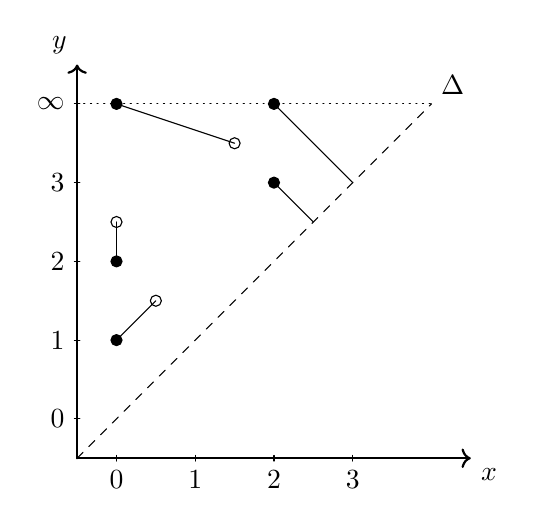
\begin{tikzpicture}[line cap=round, line join=round, x=1cm, y=1cm]
        
        \draw[thick,->] (0,0) -- (5,0) node[anchor=north west] {$x$};
        \draw[thick,->] (0,0) -- (0,5) node[anchor=south east] {$y$};
        \draw[dashed] (0,0) -- (4.5,4.5) node[above right] {$\Delta$};
        \draw[dotted] (0,4.5) -- (4.5,4.5);

        \draw (0.5 cm,1pt) -- (0.5 cm,-1pt) node[anchor=north] {0};
        \draw (1.5 cm,1pt) -- (1.5 cm,-1pt) node[anchor=north] {1};
        \draw (2.5 cm,1pt) -- (2.5 cm,-1pt) node[anchor=north] {2};
        \draw (3.5 cm,1pt) -- (3.5 cm,-1pt) node[anchor=north] {3};

        \draw (1pt,0.5 cm) -- (-1pt,0.5 cm) node[anchor=east] {0};
        \draw (1pt,1.5 cm) -- (-1pt,1.5 cm) node[anchor=east] {1};
        \draw (1pt,2.5 cm) -- (-1pt,2.5 cm) node[anchor=east] {2};
        \draw (1pt,3.5 cm) -- (-1pt,3.5 cm) node[anchor=east] {3};

        \draw (1pt,4.5 cm) -- (-1pt,4.5 cm) node[anchor=east] {$\infty$};

        \draw[fill=black] (0.5, 1.5) circle (2pt); 
        \draw[fill=black] (0.5, 2.5) circle (2pt); 
        \draw[fill=black] (0.5, 4.5) circle (2pt); 

        \draw[fill=black] (2.5, 3.5) circle (2pt); 
        \draw[fill=black] (2.5, 4.5) circle (2pt);
        
        \draw[] (1, 2) circle (2pt);
        \draw[] (0.5, 3) circle (2pt);
        \draw[] (2, 4) circle (2pt);

        \draw (0.5, 3) -- (0.5, 2.5);
        \draw (1, 2) -- (0.5, 1.5);
        \draw (0.5, 4.5) -- (2, 4);
        \draw (2.5, 4.5) -- (3.5, 3.5);
        \draw (2.5, 3.5) -- (3, 3);
        
    \end{tikzpicture}
    \caption{Wasserstein distance between two persistence diagrams.}
\end{figure}
\end{frame}

\section{Structure Theorem}

\begin{frame}
  \frametitle{Structure Theorem}
  \begin{block}{Theorem}
    Let $ (V, \pi) $ be a persistence module. There exist a barcode $ \barc(V, \pi) $, with $ \mu \colon \barc (V, \pi) \longrightarrow \mathbb N $, the multiplicity of the barcode intervals, such that there is a unique direct sum decomposition
    \begin{align}
        V \cong \bigoplus_{I \in  \barc (V)} \mathbb F (I)^{\mu (I)}. \label{eq:structure}
    \end{align}
  \end{block}
\end{frame}

\section{Stability Theorems}

\subsection{Interleaving Stability Theorem}

\begin{frame}
  \frametitle{Stability Theorems}
  \framesubtitle{Interleaving Stabiltiy Theorem}
  
  \begin{block}{Theorem}
    There is an isometry between a persistence module with the interleaving distance and its barcode with the bottleneck distance. That is, given two persistence modules $ V $ and $ W $, it holds that
    \begin{equation}
        \di (V, W) = \db (\barc(V), \barc(W)).
    \end{equation} 
  \end{block}
\end{frame}

\subsection{Hausdorff Stability Theorem}

\begin{frame}
  \frametitle{Stability Theorems}
  \framesubtitle{Hausdorff Stability Theorem}
  \begin{block}{Theorem}
    Let $ X $ be a triangulable space, and $ f, g\colon X \to \R $ continuous tame functions. Then,
    \begin{align}
        \db (D(f), D(g)) \leq \dhf(D(f), D(g)) \leq \|f-g\|_\infty.
    \end{align}
  \end{block}
\end{frame}

\subsection{Gromov-Hausdorff Stability Theorem}

\begin{frame}
  \frametitle{Stability Theorems}
  \framesubtitle{Gromov-Hausdorff Stability Theorem}

  \begin{block}{Theorem}
    Let $ (X, d_X) $, $ (Y, d_Y) $ be finite metric spaces. Then, for any $ k \in \N$, 
    \begin{equation}
        \db( D_k(\rf(X, d_X)), D_k(\rf(Y, d_Y))) \leq \dgh((X, d_X), (Y, d_Y)).
    \end{equation}
  \end{block}

\end{frame}

\section{Vectorizations}
\subsection{Persistence landscapes}

\begin{frame}
  \frametitle{Vectorizations}
  \framesubtitle{Persistence landscapes}
  \begin{block}{Definition (Rank function)}
    The {\bf rank function} of a persistence module $ V $ is the function $ \delta \colon \R^2 \to \R $ given by
    \begin{equation}
        \lambda(b, d) = \begin{cases}
            \beta_b^d &\text{ if }  b \leq d, \\
            0 &\text{ otherwise}.
        \end{cases}
    \end{equation}
  \end{block}
  \pause
  \begin{block}{Definition (Persistence landscape)}
    A {\bf persistence landscape} is a function $ \lambda \colon \N \times \R \to \overline \R $, defined as
    \begin{equation}
        \lambda(k, t) \coloneq \sup \{ m \geq 0 \mid \beta^{t-m, t+m} \geq k\}.
    \end{equation}
  \end{block}
\end{frame}

\begin{frame}
  \begin{figure}
        \centering
        \begin{subfigure}[b]{0.25\linewidth}
            \centering
            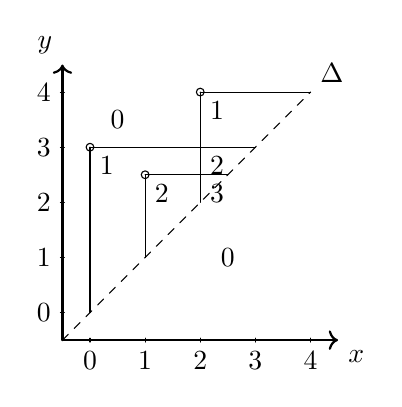
\begin{tikzpicture}[line cap=round, line join=round, x=1cm, y=1cm, scale=0.7]
                
                \draw[thick,->] (0,0) -- (5,0) node[anchor=north west] {$x$};
                \draw[thick,->] (0,0) -- (0,5) node[anchor=south east] {$y$};
                \draw[dashed] (0,0) -- (4.5,4.5) node[above right] {$\Delta$};

                \draw (0.5 cm,1pt) -- (0.5 cm,-1pt) node[anchor=north] {0};
                \draw (1.5 cm,1pt) -- (1.5 cm,-1pt) node[anchor=north] {1};
                \draw (2.5 cm,1pt) -- (2.5 cm,-1pt) node[anchor=north] {2};
                \draw (3.5 cm,1pt) -- (3.5 cm,-1pt) node[anchor=north] {3};
                \draw (4.5 cm,1pt) -- (4.5 cm,-1pt) node[anchor=north] {4};

                \draw (1pt,0.5 cm) -- (-1pt,0.5 cm) node[anchor=east] {0};
                \draw (1pt,1.5 cm) -- (-1pt,1.5 cm) node[anchor=east] {1};
                \draw (1pt,2.5 cm) -- (-1pt,2.5 cm) node[anchor=east] {2};
                \draw (1pt,3.5 cm) -- (-1pt,3.5 cm) node[anchor=east] {3};
                \draw (1pt,4.5 cm) -- (-1pt,4.5 cm) node[anchor=east] {4};

                \draw (1.5, 3) circle (2pt) node[below right] {2};
                \draw (0.5, 3.5) circle (2pt) node[below right] {1};
                \draw (2.5, 4.5) circle (2pt) node[below right] {1};

                \draw (3, 1.5) node {0};
                \draw (1, 4) node {0};
                \draw (2.5, 3.5) node[below right] {2};
                \draw (2.5, 3) node[below right] {3};

                \draw (1.5, 3) -- (1.5, 1.5);
                \draw (1.5, 3) -- (3, 3);
                \draw (0.5, 3.5) -- (0.5, 0.5);
                \draw (0.5, 3.5) -- (3.5, 3.5);
                \draw (2.5, 4.5) -- (2.5, 2.5);
                \draw (2.5, 4.5) -- (4.5, 4.5);
                
            \end{tikzpicture}
            \caption{Rank function.}
        \end{subfigure}
        \hspace{1cm}
        \begin{subfigure}[b]{0.25\linewidth}
            \centering
            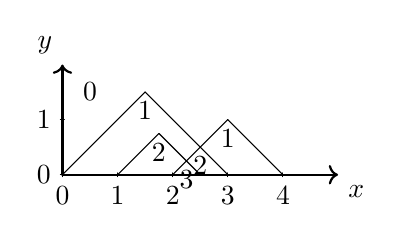
\begin{tikzpicture}[line cap=round, line join=round, x=1cm, y=1cm, scale=0.7]
                
                \draw[thick,->] (0,0) -- (5,0) node[anchor=north west] {$x$};
                \draw[thick,->] (0,0) -- (0,2) node[anchor=south east] {$y$};

                \draw (0 cm,1pt) -- (0 cm,-1pt) node[anchor=north] {0};
                \draw (1 cm,1pt) -- (1 cm,-1pt) node[anchor=north] {1};
                \draw (2 cm,1pt) -- (2 cm,-1pt) node[anchor=north] {2};
                \draw (3 cm,1pt) -- (3 cm,-1pt) node[anchor=north] {3};
                \draw (4 cm,1pt) -- (4 cm,-1pt) node[anchor=north] {4};

                \draw (1pt,0 cm) -- (-1pt,0 cm) node[anchor=east] {0};
                \draw (1pt,1 cm) -- (-1pt,1 cm) node[anchor=east] {1};

                \draw (1.75, 0.75) node[below] {2};
                \draw (1.5, 1.5) node[below] {1};
                \draw (3, 1.0) node[below] {1};

                \draw (0.5, 1.5) node {0};
                \draw (2.5, 0.5) node[below] {2};
                \draw (2.25, 0.25) node[below] {3};

                \draw (1.75, 0.75) -- (1, 0);
                \draw (1.75, 0.75) -- (2.5, 0);
                \draw (1.5, 1.5) -- (0, 0);
                \draw (1.5, 1.5) -- (3, 0);
                \draw (3, 1.0) -- (2, 0);
                \draw (3, 1.0) -- (4, 0);
                
            \end{tikzpicture}
            \caption{Rescaled rank function.}
        \end{subfigure}
        \hspace{1cm}
        \begin{subfigure}[b]{0.25\linewidth}
            \centering
            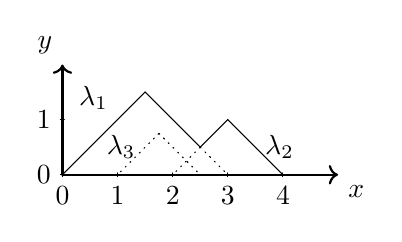
\begin{tikzpicture}[line cap=round, line join=round, x=1cm, y=1cm, scale=0.7]
                
                \draw[thick,->] (0,0) -- (5,0) node[anchor=north west] {$x$};
                \draw[thick,->] (0,0) -- (0,2) node[anchor=south east] {$y$};

                \draw (0 cm,1pt) -- (0 cm,-1pt) node[anchor=north] {0};
                \draw (1 cm,1pt) -- (1 cm,-1pt) node[anchor=north] {1};
                \draw (2 cm,1pt) -- (2 cm,-1pt) node[anchor=north] {2};
                \draw (3 cm,1pt) -- (3 cm,-1pt) node[anchor=north] {3};
                \draw (4 cm,1pt) -- (4 cm,-1pt) node[anchor=north] {4};

                \draw (1pt,0 cm) -- (-1pt,0 cm) node[anchor=east] {0};
                \draw (1pt,1 cm) -- (-1pt,1 cm) node[anchor=east] {1};

                \draw[dotted] (1.75, 0.75) -- (1, 0);
                \draw[dotted] (1.75, 0.75) -- (2.5, 0);
                \draw (1.5, 1.5) -- (0, 0);
                \draw (1.5, 1.5) -- (2.5, 0.5);
                \draw[dotted] (2.5, 0.5) -- (3, 0);
                \draw (3, 1.0) -- (2.5, 0.5);
                \draw[dotted] (2.5, 0.5) -- (2, 0);
                \draw (3, 1.0) -- (4, 0);

                \draw (1, 1) node[above left] {$\lambda_1$};
                \draw (1.5, 0.5) node[left] {$\lambda_3$};
                \draw (3.5, 0.5) node[right] {$\lambda_2$};
                
            \end{tikzpicture}
            \caption{Persistence landscape.}
        \end{subfigure}
        \caption{Persistence landscape of a persistence diagram.}
    \end{figure}
\end{frame}

\subsection{Persistence images}

\begin{frame}
  \frametitle{Vectorizations}
  \framesubtitle{Persistence images}

  \begin{block}{Definition (Persistence surface)}
    The {\bf persistence surface} associated to $ D $, by $ f $ and $ \phi_u $ is a function $ \rho_D \colon \R^2 \to \R $ defined as
    \begin{equation}
        \rho_D(z) \coloneq \sum_{u \in T(D)} f(u) \phi_u(z).
    \end{equation}
  \end{block}
  \pause
  \begin{block}{Definition (Persistence image)}
    Let $ D $ be a persistence diagram with an associated persistence surface $ \rho_D $. The {\bf persistence image} of $ D $ by $ \rho_D $ is the collection $ \rho $ of {\bf pixels}
    \begin{equation}
        I(\rho_D)_p \coloneq \iint_p \rho_B dy dx.
    \end{equation}
  \end{block}
\end{frame}

\begin{frame}
  \begin{figure}
      \centering
      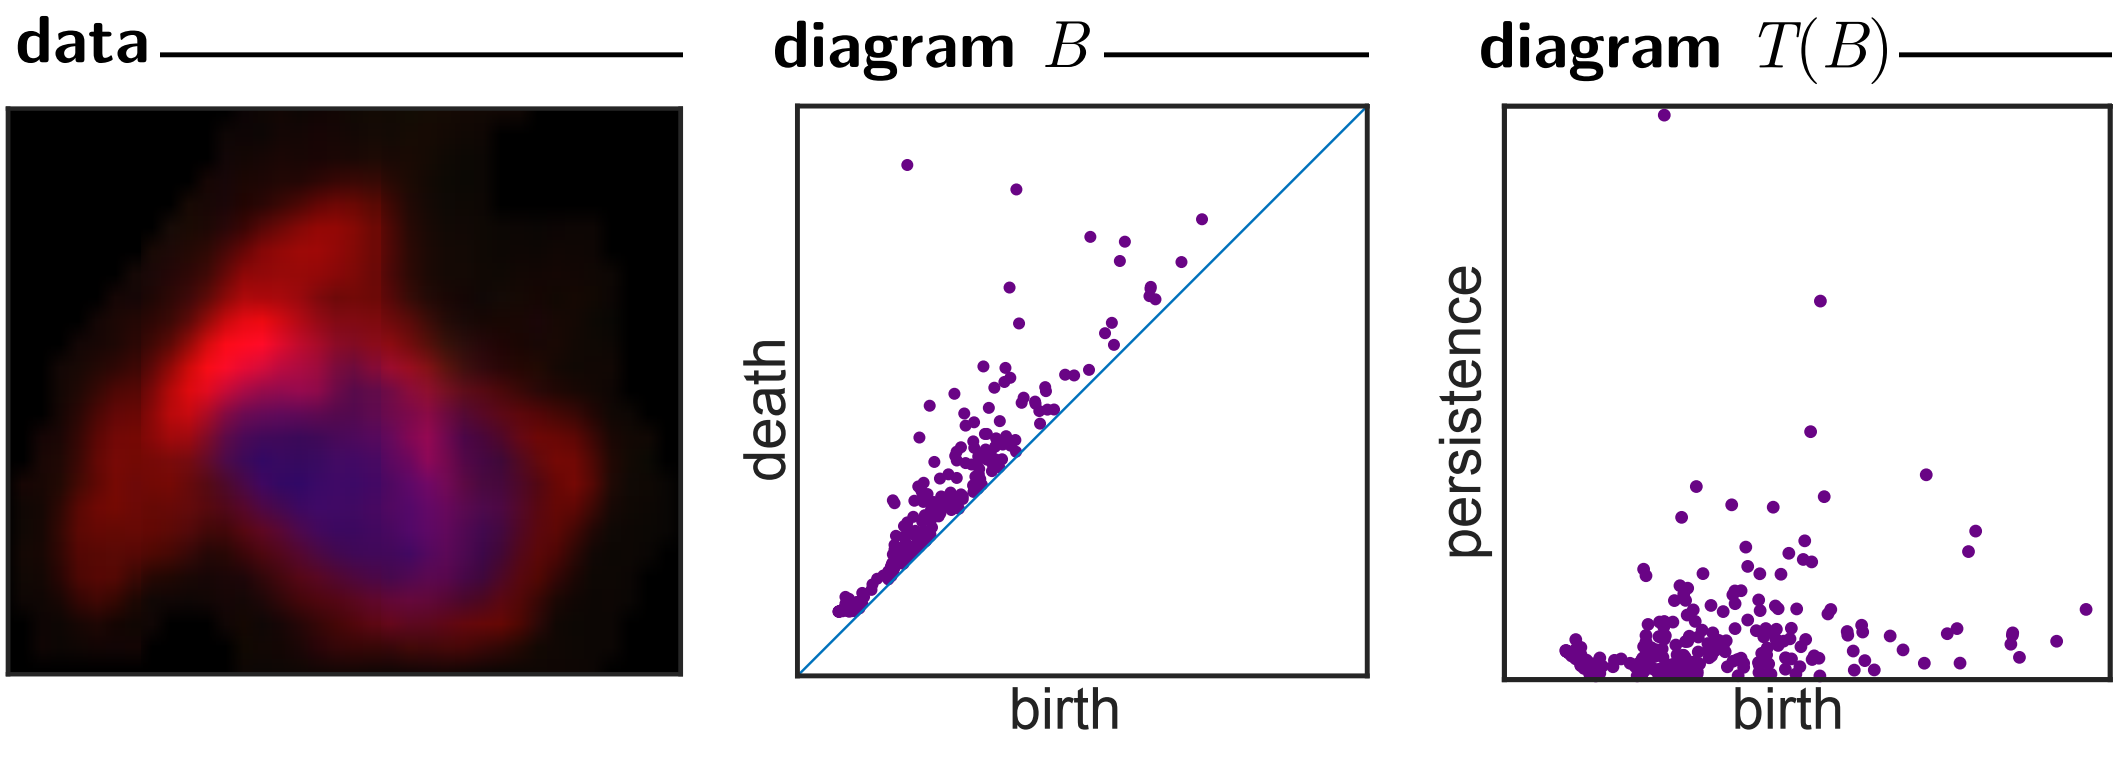
\includegraphics[width=0.66\linewidth]{../figures/persistence-images-1.png}
      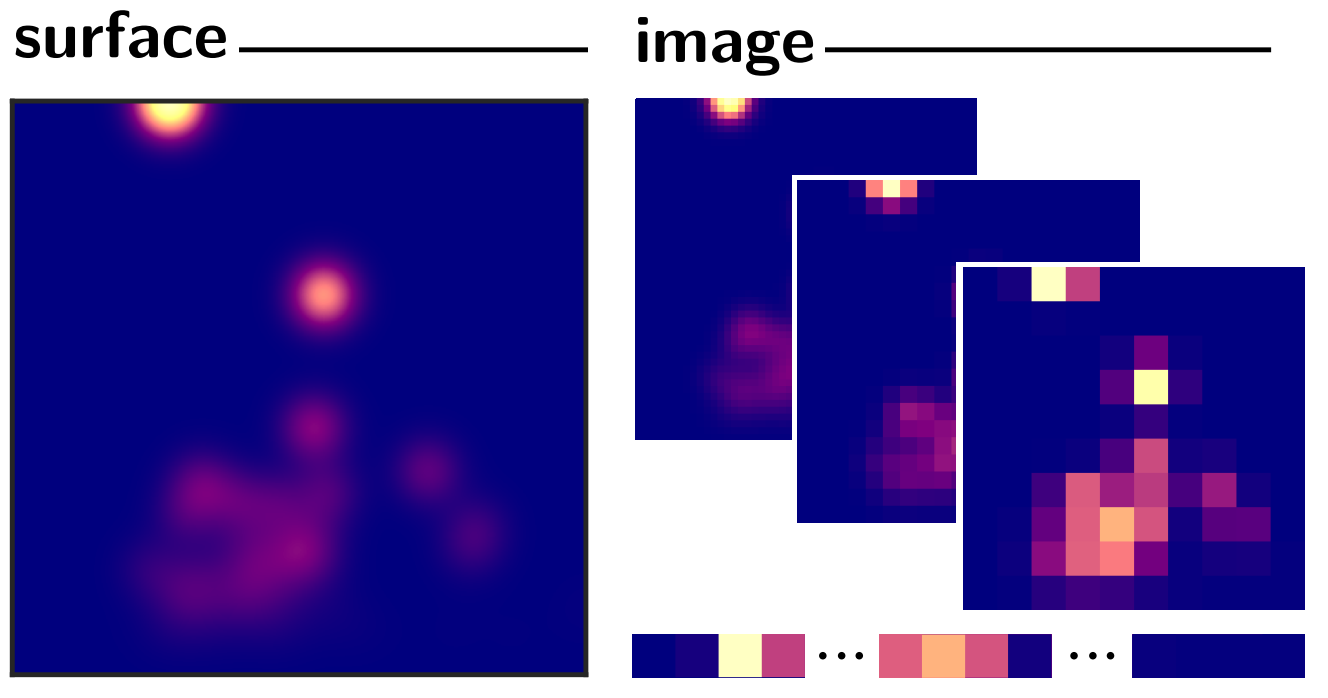
\includegraphics[width=0.44\linewidth]{../figures/persistence-images-2.png}
      \caption{Algorithm pipeline to transform data into a persistence image.}
    \end{figure}
\end{frame}

\subsection{Euler curves}

\begin{frame}
  \frametitle{Vectorizations}
  \framesubtitle{Euler curves}
  \begin{block}{Definition}
      Let $ K $ be a simplicial complex, and let $ K^p $ be its $p$-skeleton. The {\bf Euler characteristic} of $ K $ is the alternating sum of the number of cells in its dimension
      \begin{equation}
          \chi(K) \coloneq \sum_d (-1)^d \#(K^d).
      \end{equation}
  \end{block}
  \pause
  \begin{block}{Definition}
      Let $ K $ be a simplicial complex. Let $ f \colon K \to \R $ be a filtration function. The {\bf Euler characteristic curve} is a function that assign an Euler characteristic $ \chi $ for each filtration level $ t \in \R $. 
      \begin{equation}
          \ecc(K, t) \coloneq \chi(K_t),
      \end{equation}
      where $ K_t = f^{-1} (-\infty, t] $.
  \end{block}
\end{frame}

\begin{frame}[plain]

\begin{center}

  \bigskip  \bigskip

  \begin{Large} \textcolor{green}{\textbf{\projecttitle}} \end{Large} \bigskip \bigskip

  \begin{footnotesize} \textrm{Master's Final Thesis} \\ \end{footnotesize} \bigskip \bigskip

  \begin{footnotesize} \textbf{Mathematics and Applications Master} -- Curse 2024 - 2025 \end{footnotesize} \bigskip \bigskip

  \begin{footnotesize} \textsf{Author:} \textit{\authorname} \\
  \smallskip \textsf{Advisor (UPM):} \textit{Jaime Santos Rodríguez} \\
  \smallskip \textsf{Advisor (UAM):} \textit{Lui Guijarro Santamaría} \\
\end{footnotesize} \bigskip \bigskip


  
\includegraphics[height=1cm]{../figures/marcaUAM_AhorizontalColor_imp.pdf}

\end{center}

\end{frame}

\end{document}